%Discuss the design of your experiments, the results you obtained,and how they help in evaluating the claims you made in the introduction. You may also use the evaluation results in this section to justify your design choices or assess the contributions of different aspects of your design towards the overall goals.

The result section of the report is divided into two parts. In the first part, the outcome of the data mining is shown under the section exploratory data analysis. In the second section performance of the models are noted down. 

\subsection{Exploratory data analysis}

\subsubsection{Dataset}\hspace*{\fill} \\
The data extraction method mentioned in the section~\ref{sec: Design} was followed to generate the dataset from the historical company information.

To prepare this dataset, the historical data from 2011 to 2021 is considered. During the considered period, a company would generally have multiple status reports, however, to get the latest updates of each company the last report was considered. The reports are also filtered out based on the report type as not all reports would have all the required information. 

The data extraction and feature engineering processes are very time-consuming. To make sure these processes run within an acceptable time and to support our design method, 25\% majority classes were not included while preparing the dataset. From the paper on SMOTE~\cite{2002}, we have seen the under-sampling with SMOTE performs relatively well. So theoretically the performance will still get improvement.

In the generated dataset, there are a total of 30 columns available. Out of which three columns are report date, report id, these three columns were dropped before the training. However, these columns are used for identifying the company information after the training. 

 27 columns were selected as the features, the remaining one column contains the class information, which was used for the training label.  

The total number of instances is 48,549. Among this data, only 1358 are marked suspicious companies. As mentioned earlier the actual data was filtered to avoid duplicated and inadequate reports. 
\begin{itemize}
    \item Total number of columns: 30
    \item Number of company entries: 48,539
    \item Target label: Suspicious
    \item Total Features: 27
    \item Total suspicious cases: 1358
\end{itemize}


\subsubsection{Class Distribution}\hspace*{\fill} \\
From the initial assessment we can see the that classes are very imbalanced. In the dataset there is only 1358 fraudulent cases out of 48,549 ones. That means only 2.8\% of companies are fraudulent or specious [shown in figure~\ref{fig:class distribution}]. However as mentioned in the dataset section above, 25\% of majority class were under samples during the dataset preparation. That means the actual class distribution is much lower in reality. However to make a realistic model, we will consider this class distribution in the rest of the paper. 

\begin{figure}[H]
    \centering
    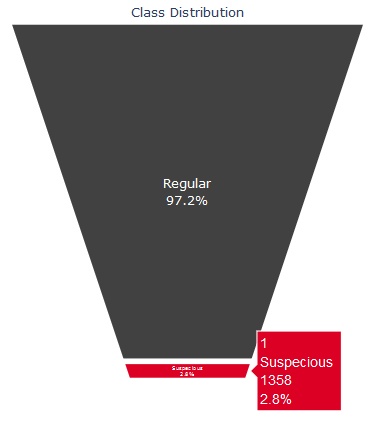
\includegraphics[width=.8\linewidth]{figures/class_imbalance.png}
    \caption{Class Distribution}
    \label{fig:class distribution}
\end{figure}

Even after the undersampling of the majority class, we can see from figure~\ref{fig:class distribution} that our dataset is highly imbalanced. Hence during the training of different models, we had to try different sampling methods to feed the model with a similar class distribution. In the model performance section with and without SMOTE is shown. 

\subsubsection{Task complexity}\hspace*{\fill} \\
From the class distribution, we can already assume that classifying suspicious classes would be extremely hard. To understand the complexity more, dimension reduction functions were applied to visualize the class distribution in a two-dimensional space. As we can find the figure~\ref{fig:Dimension reduction}, the classes cannot be easily separated. So the classes are not only imbalanced but also closely related. That means complexity to build a model to detect suspicious class would be a huge challenge.
 
\begin{figure}[H]
    \centering
    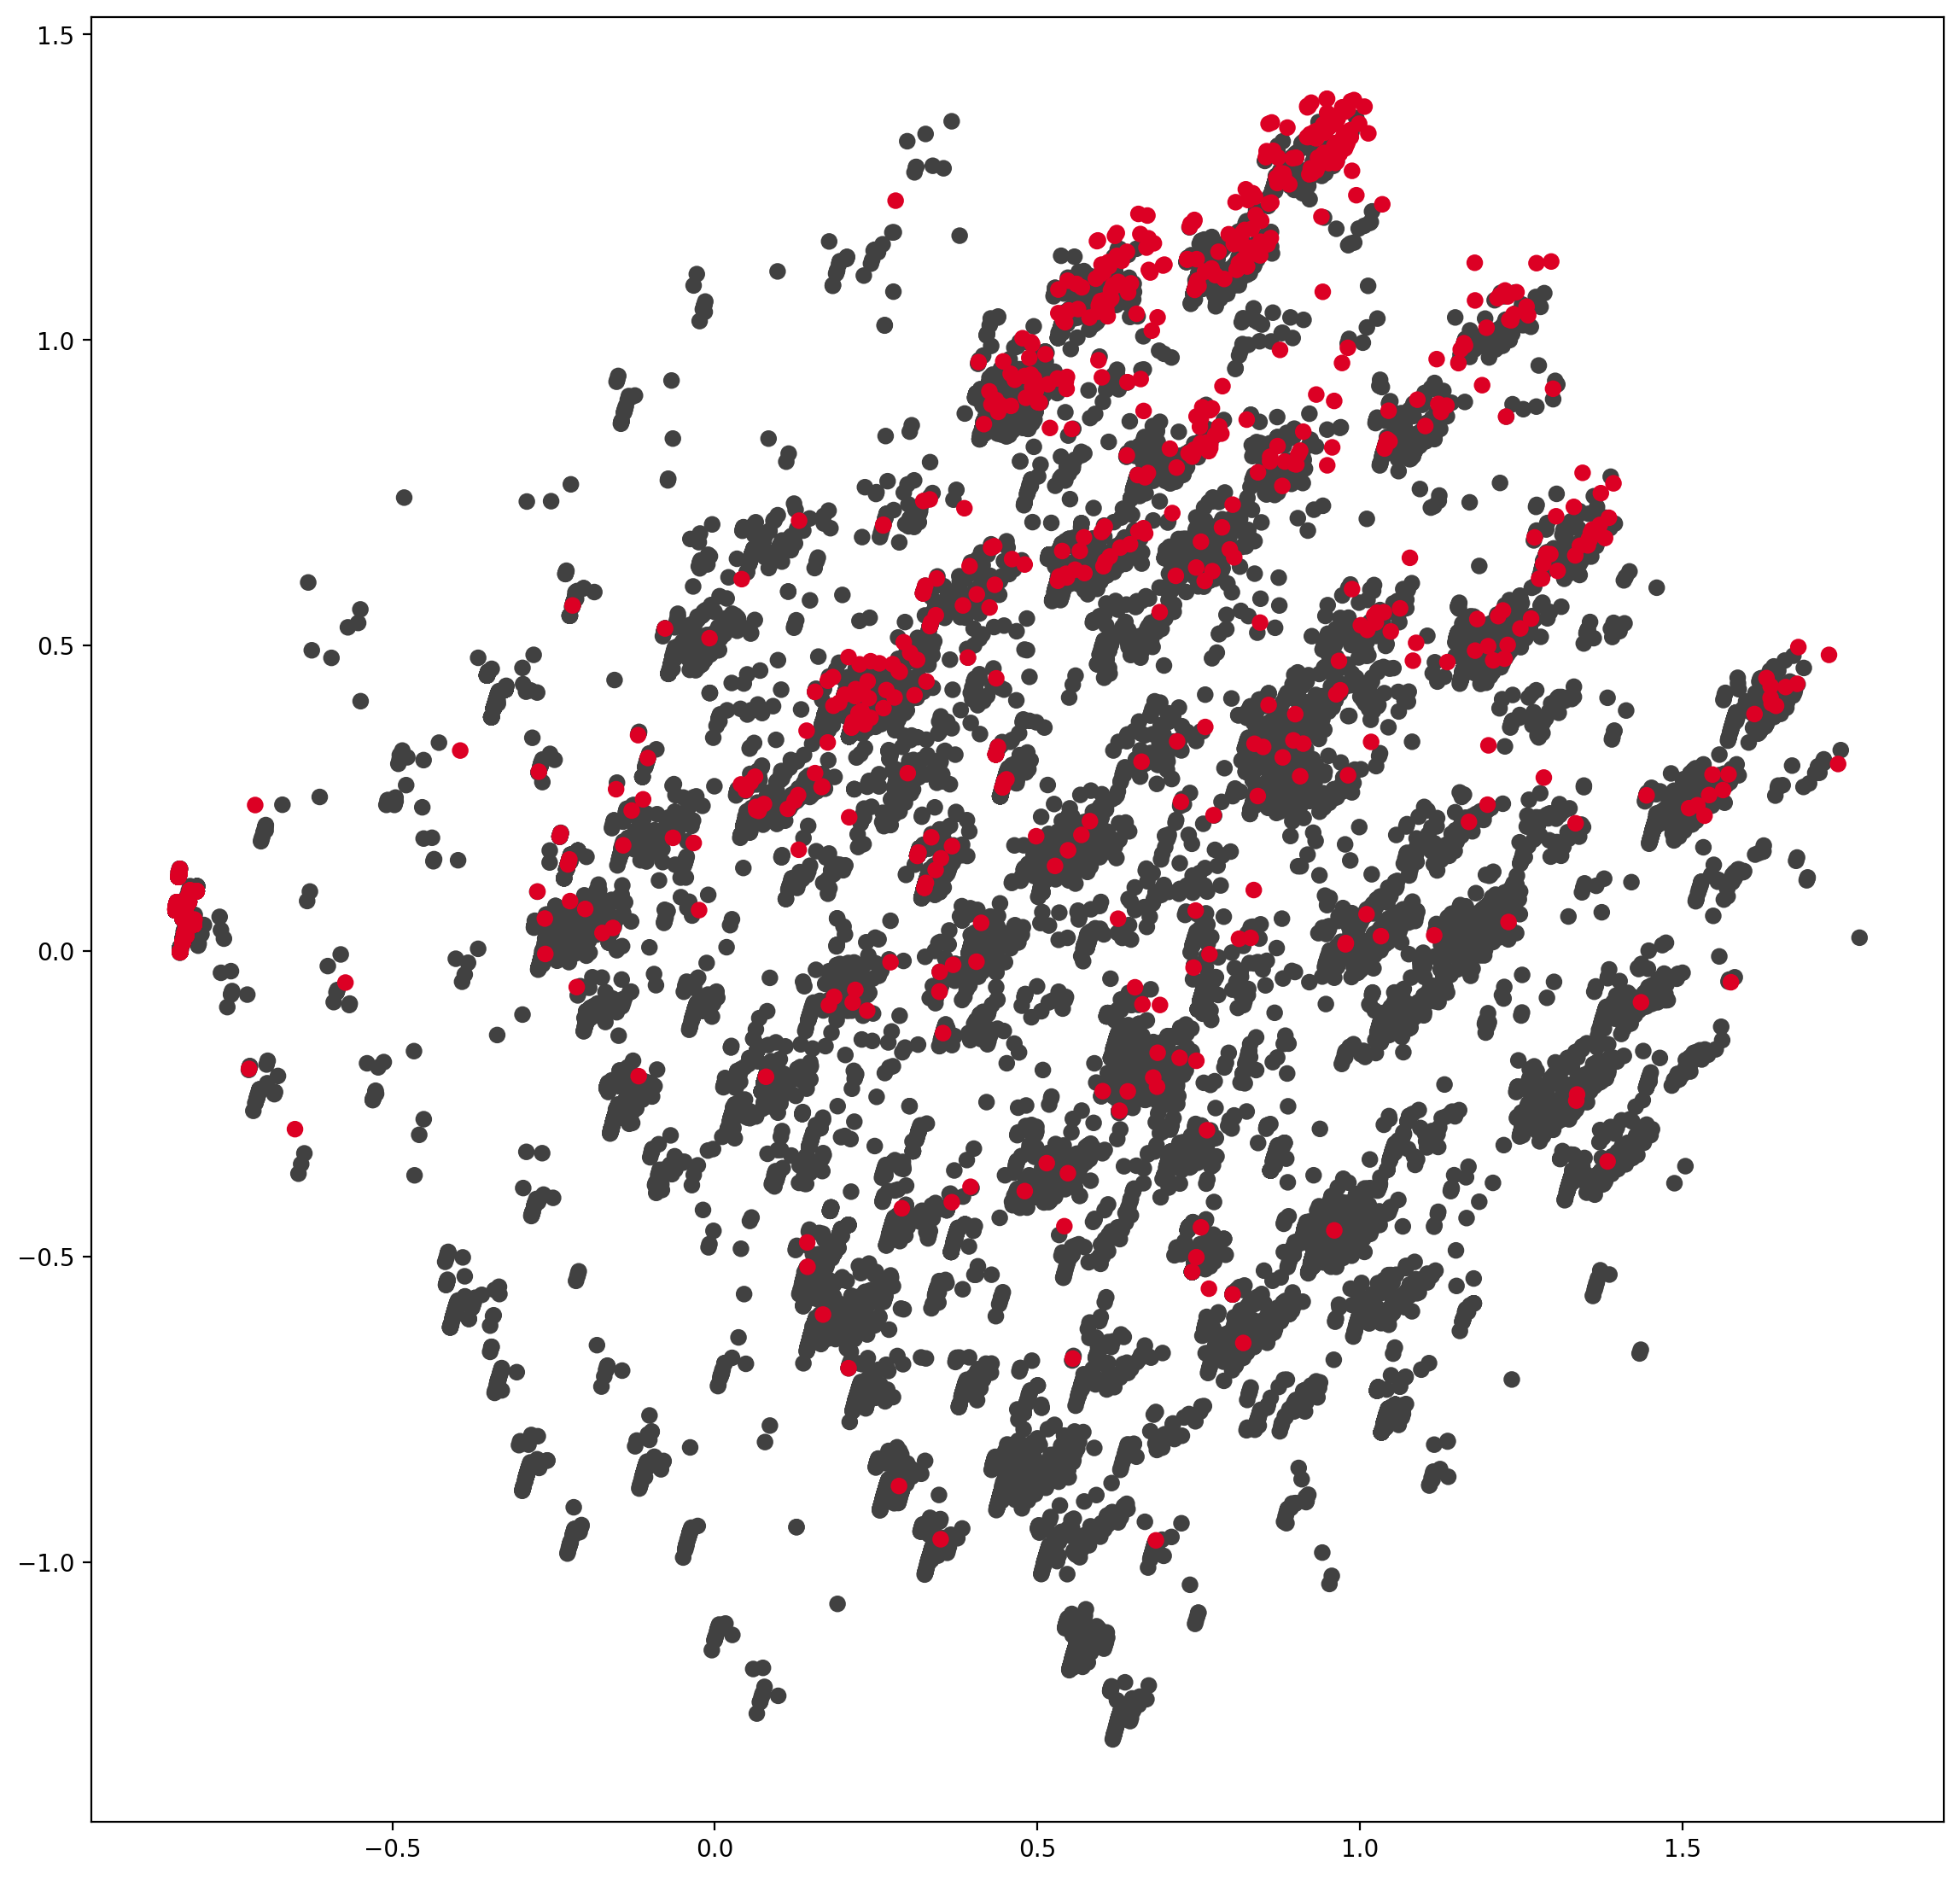
\includegraphics[width=\linewidth]{figures/pca_2d.png}
    \caption{Classes after Dimension reduction}
    \label{fig:Dimension reduction}
\end{figure}


\subsubsection{Class Proportion}\hspace*{\fill} \\
 It is important to understand the effectiveness of the selected features. Theoretically, we want to select the features which have the indication of suspicious patterns. To do so, the proportion of the classes based on features were prepared. In the figure~\ref{fig:feature proportion} the proportion of the binary features are shown.
\begin{figure}[H]
    \centering
    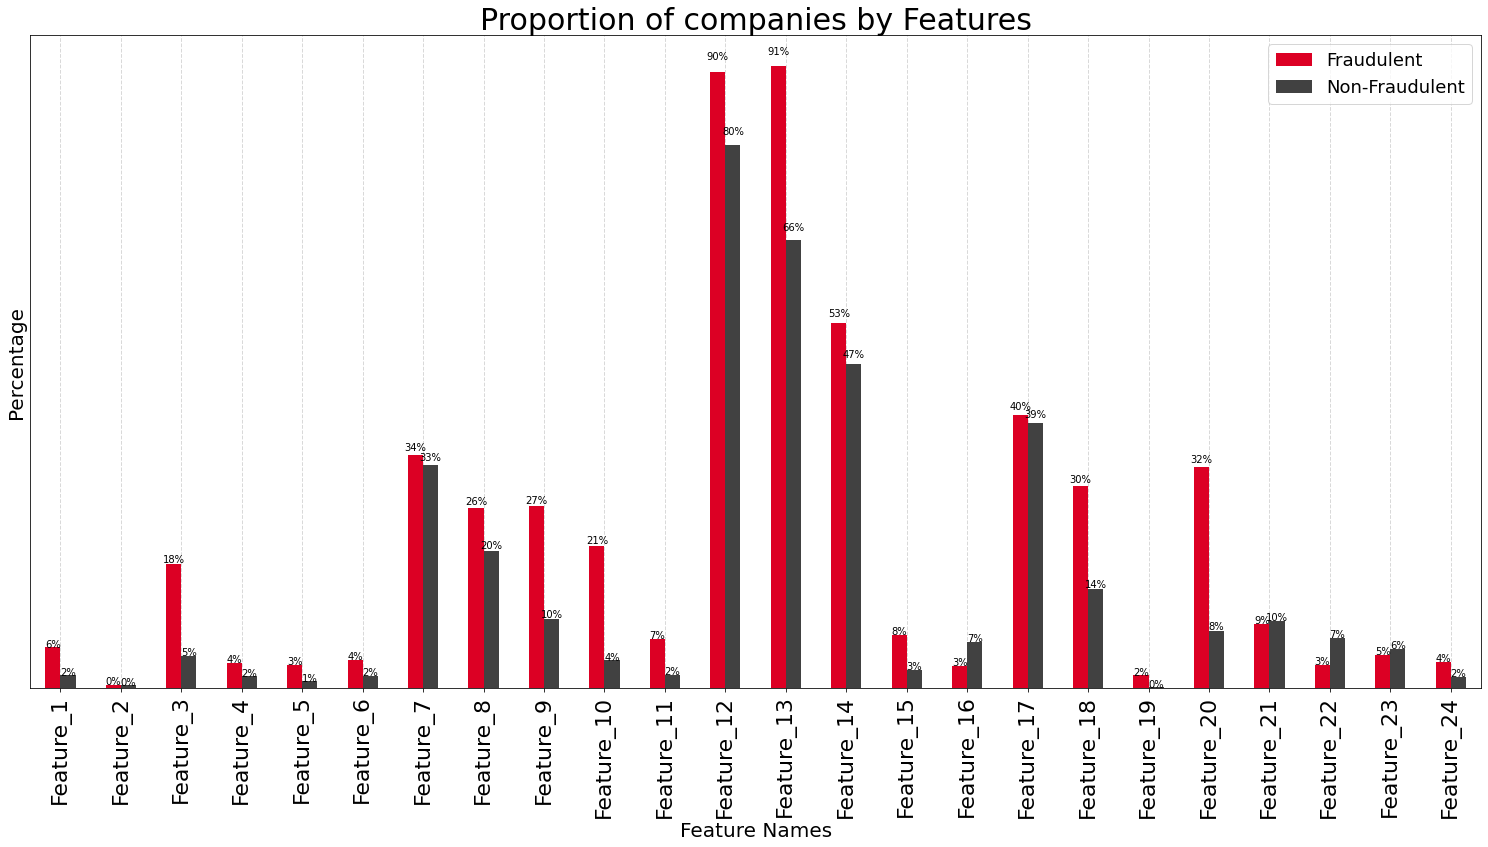
\includegraphics[width=\linewidth]{figures/feature_proportion.png}
    \caption{Proportion of binary features}
    \label{fig:feature proportion}
\end{figure}

From the figure~\ref{fig:feature proportion} we can see that majority of the engineered features has a higher proportion of suspicious classes than regular classes. This is a good indication that the selected features may help the model classify the patterns. 


For the continues variable statistical information like mean, median and standard deviation between two classes were considered to find the effectiveness of the features. The figure~\ref{fig:Continues Feature Statistics} shows the statistics of the continues variable features. 

\begin{figure}[H]
    \centering
    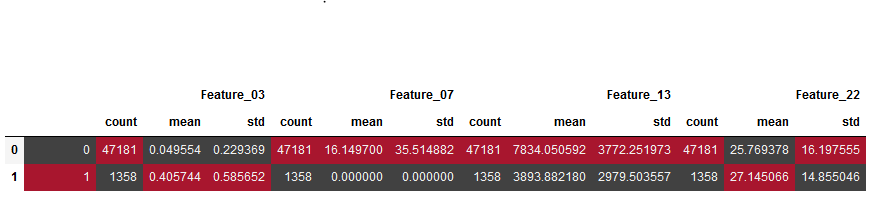
\includegraphics[width=\linewidth]{figures/feature_proportion_2.PNG}
    \caption{Continues Feature Statistics}
    \label{fig:Continues Feature Statistics}
\end{figure}


\subsubsection{Correlation Matrix}\hspace*{\fill} \\
A good visualization tool to understand the relation between classes and features is the correlation matrix. In figure~\ref{fig:corr} we can visualize the relation between suspicious class and respective features. At a glance, we can see that the correlation between features and classes are very low. That is a good reference to understand the complexity of the tasks. 
\begin{figure}[H]
    \centering
    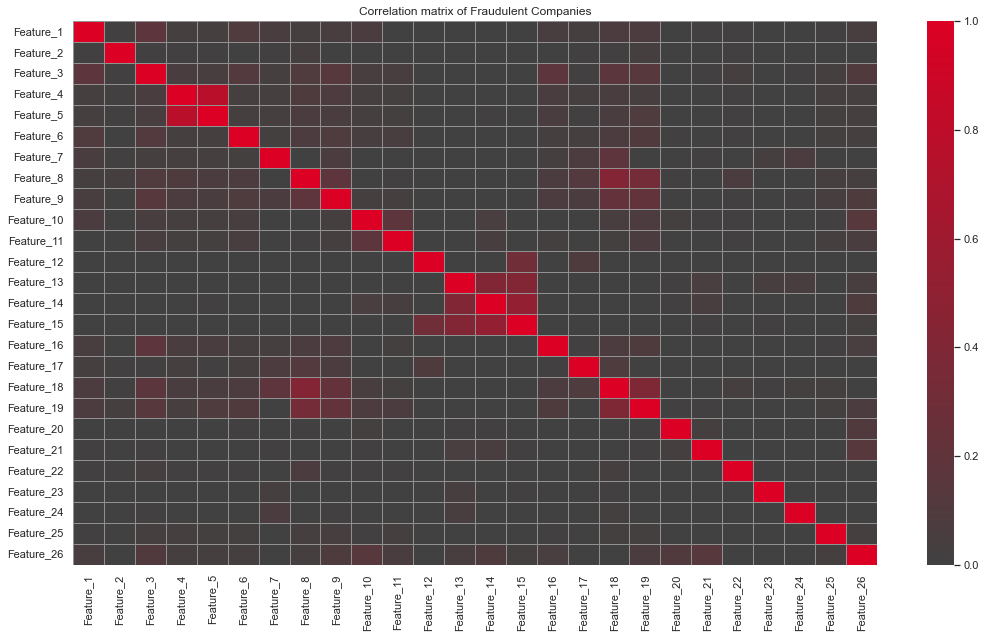
\includegraphics[width=\linewidth]{figures/corr.png}
    \caption{Correlation Matrix}
    \label{fig:corr}
\end{figure}

\subsection{Model Performance Results}\label{sec: model results}

To select the right classifier, it is important to verify the performance of each model by using all types of performance matrices. For this paper to select we will use the mentioned method in the section Tools of trades in the Design Overview section. The below subsections provide the performance of each model in different matrices. 


There is a total of six models we have selected for comparison. We have random foreset, XGBoost, and artificial neural networks models and their variation with SMOTE. 

\subsubsection{Performance Metrics:}\hspace*{\fill} \\
In the table~\ref{tab:per_res} the performance results of Random Forest, XGBoost, and Artificial Natural networks are shown. Each model has with and without SMOTE version. Each models performance results are shown in the respective rows. The columns show, accuracy, precision, recall and f1-score for each respective model over the test dataset. 
\begin{table}[H]
    \begin{tabular}{clrrrr}
    \cline{1-6}
    \multicolumn{1}{l}{SMOTE} & Model         & \multicolumn{1}{l}{Accuracy} & \multicolumn{1}{l}{Precision} & \multicolumn{1}{l}{Recall} & F1 \\ \cline{1-6} 
    \multirow{3}{*}{No}       & Random Forest &0.97  & 0.42  & 0.07  & 0.11 \\
                              & XGBoost       &0.97  & 0.44  & 0.03  & 0.06 \\
                              & ANN           &0.97  & 0.30  & 0.10  & 0.15 \\ \cline{1-6} 
    \multirow{3}{*}{Yes}       & Random Forest &0.88  & 0.11  & 0.47  & 0.17 \\
                              & XGBoost       &0.88  & 0.10  & 0.47  & 0.17 \\
                              & ANN           &0.86  & 0.09  & 0.46  & 0.15 \\ \cline{1-6} 
    \end{tabular}
    \caption{Test Data performance}
    \label{tab:per_res}
\end{table}


The figure~\ref{fig:test_train} shows the performance results of each model in bar charts. The columns show the f1-performance results of each model. The bars are clustered into performance results of train and test datasets. 

\begin{figure}[H]
    \centering
    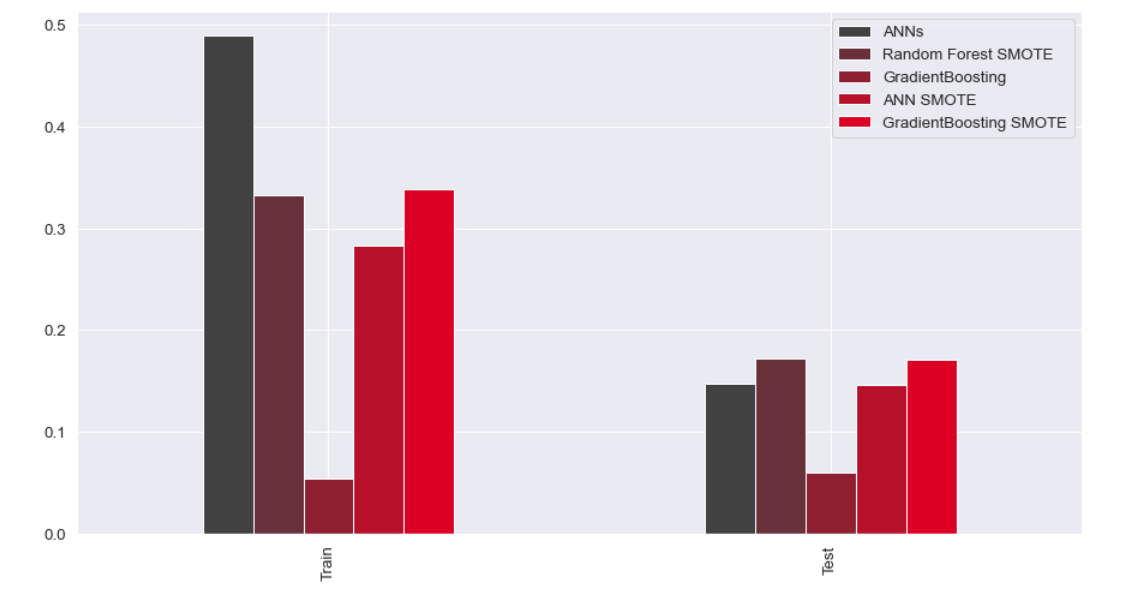
\includegraphics[width=\linewidth]{figures/results.PNG}
    \caption{Performance over train and test data}
    \label{fig:test_train}
\end{figure}

\subsubsection{ROC curve}\hspace*{\fill} \\
Figure~\ref {fig:roc_all} shows the ORC curves of all the models in a single place. The x-axis indicates the false positive rate, and the y-axis indicates the true positive rate. The ROC curves are placed together in this figure for visual comparison. 
\begin{figure}[h]
    \centering
    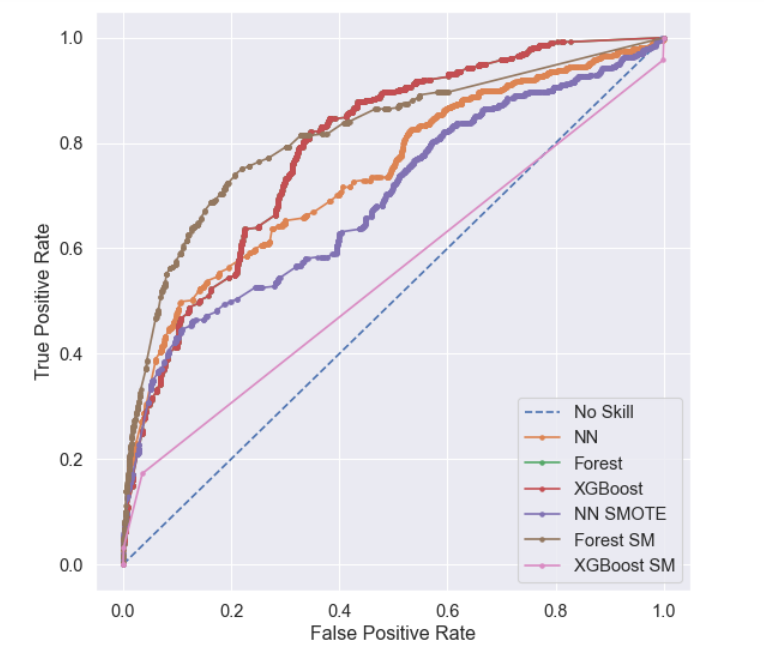
\includegraphics[width=\linewidth]{figures/roc_res.PNG}
    \caption{ROC Curves}
    \label{fig:roc_all}
\end{figure}

In the figure~\ref{fig:roc_all_2} ROC curves are displayed in comparison with no skill classifiers. This gives a visual demonstration of the area under the curve. 
\begin{figure}[h]
    \centering
    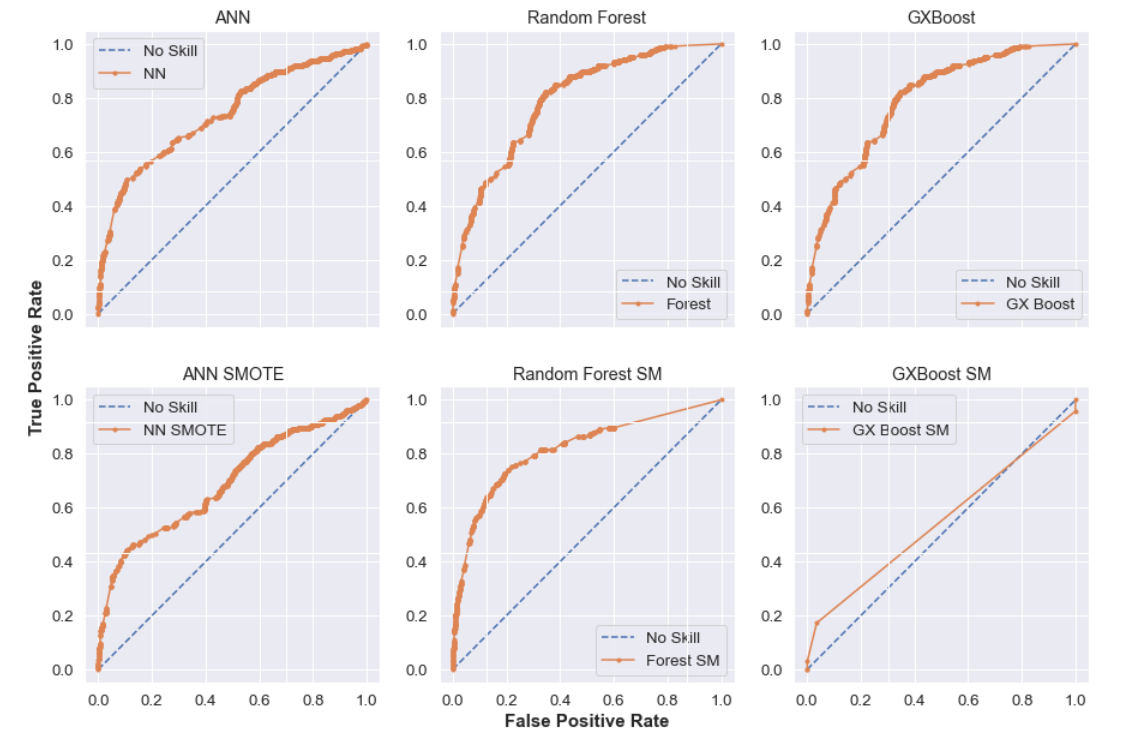
\includegraphics[width=\linewidth]{figures/roc_res_full.PNG}
    \caption{ROC Curves compare to no skill model}
    \label{fig:roc_all_2}
\end{figure}


% \mytodo{model selection hint\: %https://medium.com/@matteding/imbalanced-data-fraud-detection-3185c1cdaa77}

\subsubsection{AUC ROC}\hspace*{\fill} \\
AUC ROC Curve means the area under the ROC curve. The AUC ROC values for each model is shown in the table~\ref{tab: roc_auc}. The values help us to choose the best model when it's difficult to see from the ROC curve visually. 
\begin{table}[H]
    \begin{tabular}{|l|l|}
    \hline
    MODEL     & ROC AUC \\ \hline
    No Skill  & 0.500   \\ \hline
    ANN       & 0.742   \\ \hline
    RF        & 0.793   \\ \hline
    XG        & 0.725   \\ \hline
    ANN SMOTE & 0.693   \\ \hline
    RF SMOTE  & 0.817   \\ \hline
    XG SMOTE  & 0.549   \\ \hline
    \end{tabular}
    \caption{ROC AUC Values}
    \label{tab: roc_auc}
\end{table}


\subsubsection{Confusion Matrix}\hspace*{\fill} \\
In the figure~\ref{fig:cm_rf} the performance of the random forest with SMOTE is shown in a form of a confusion matrix. In the matrix predicted labels and trues labels are shown in a 2 by 2 matrix. The bottom right box shows the True positive cases on the other the top right shows the false-positive results on the test data. 
\begin{figure}[H]
    \centering
    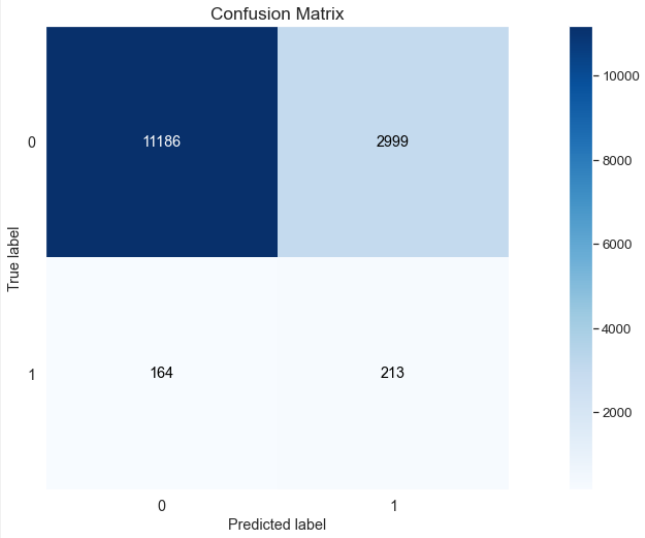
\includegraphics[width=\linewidth]{figures/cm.PNG}
    \caption{Confusion Matrix Random Forest}
    \label{fig:cm_rf}
\end{figure}


\subsubsection{Threshold value}\hspace*{\fill} \\
To verify the performance of the model is also important to see how the performance of the model works in the different thresholds. Figure~\ref{fig:cm_r} shows all the values of the random forest model. The thresholds values chosen for the model are 0.1, 0.15, 0.2, 0.25, 0.35, 0.4, 0.45 and 0.5. 